\chapter{Interdire la copie, ou l'encourager : l'incohérence du système actuel}

Nous avons vu dans le chapitre précédent que la copie est une action naturelle que nous exerçons tous tout à long de notre vie.
Cependant, la société ne se positionne pas forcément dans ce sens, et prend une position incohérente par rapport à la copie.
Nous allons voir pourquoi dans ce chapitre.

\section{Brevet et droit d'auteur}

Nous n'allons pas aborder de manière exhaustives les notions de brevet et de droit d'auteur, car ce sont des notions complexes qui touchent beaucoup de domaines, et qui varient en fonction du pays étudié.
Je vais par contre tâcher de les définir de manière suffisante pour pouvoir les intégrer à notre réflexion sur la copie.
Sauf si je le précise explicitement, je parlerai surtout en me basant sur la législation française.

Commençons par le droit d'auteur (ou son équivalent américain, le <<~copyright~>>).
<<~Le droit d'auteur est l'ensemble des prérogatives exclusives dont dispose un auteur ou plus généralement ses ayants droit (société de production, héritiers) sur des œuvres de l'esprit originales.~>>\footnote{Source : \url{https://fr.wikipedia.org/wiki/Droit_d\%27auteur}}

Ici, on parle donc bien <<~d'œuvres de l'esprit~>>, donc immatérielles.
Bien souvent, ces idées vont être matérialisées, et placées sur des supports (papier, DVD, \dots{}) dont on ferra commerce.
Le problème, c'est que ce modèle est lucratif pour ceux qui fabriquent les objets (libraires et imprimeurs, dans l'exemple du livre) ; il n'y a finalement pas de raison spontanée première pour que ceux-ci décident de rémunérer les auteurs des œuvres qu'il exploitent.

L'idée du droit d'auteur c'est de dire que si on fait commerce de la matérialisation de l'œuvre de quelqu'un, on lui doit un pourcentage.
La démocratisation de ce mécanisme en France est souvent attribuée à Beaumarchais, qui, en temps que dramaturge, voulait toucher un pourcentage sur la recette perçu par les comédiens qui jouaient ses pièces.

On peut diviser le droit d'auteur en deux branches :
\begin{itemize}
\item \textbf{le droit moral}, qui reconnaît à l'auteur la paternité de l'œuvre et qui vise aussi le respect de l'intégrité de l'œuvre ;
\item \textbf{les droits patrimoniaux}, qui confèrent un monopole d'exploitation économique sur l'œuvre, pour une durée variable (selon les pays ou cas) au terme de laquelle l'œuvre entre dans le domaine public \textit{(nous reviendrons sur la notion de domaine public en même temps que l'explication sur les brevets)}.
\end{itemize}\bigskip

L'auteur peut jouir de ces deux droits automatiquement, dès le moment où il a créé une œuvre.
Le droit d'auteur était à la base prévu pour durer un maximum de 5 ans.
De nos jours, on parle plutôt de 70 ans après la mort de l'auteur !

On peut déjà entrapercevoir les limites d'un tel système : à partir de quand une œuvre de l'esprit, une idée, peut être appartenir à quelqu'un ?
Comme je l'ai argumenté dans le premier chapitre, il est difficile de s'approprier quelque chose d'immatériel dans le sens où cette chose n'a souvent pas de limite clairement identifiable.
D'un autre côté, ce système est une solution qui a été trouvée pour nourrir les artistes qui produisent des œuvres immatérielles.

Cependant, on constate de plus en plus de cas où le droit d'auteur est utilisé pour protéger l'artiste contre son public (parfois même à l'insu de l'artiste), chose pour laquelle il n'a pas été prévu du tout à la base.
Mais nous y reviendrons par la suite\dots{}

L'autre <<~entrave~>> à la copie est le brevet (ou son équivalent américain, le <<~patent~>>).
<<~Un brevet est un titre de propriété industrielle qui confère à son titulaire non pas un droit d'exploitation, mais un droit d'interdiction de l'exploitation par un tiers de l'invention brevetée, à partir d'une certaine date et pour une durée limitée (20 ans en général).~>>\footnote{Source : \url{https://fr.wikipedia.org/wiki/Brevet}}

Contrairement au droit d'auteur qui est automatique, il faut faire une demande pour obtenir un brevet, ce qui a un coût (très important pour un particulier).
Un brevet n'est valable que dans un État donné.
Il est cependant possible de déposer un brevet auprès de plusieurs États, mais le coût en est multiplié et sa validation n'est pas assurée partout, car les organismes de validations sont indépendants (certains organismes peuvent délivrer des brevets valables dans plusieurs États).
Les brevet sont plutôt réservés aux inventions et aux techniques industrielles.

Pour être brevetable, une invention doit correspondre à trois critères :
\begin{enumerate}
\item Elle doit être nouvelle, c'est-à-dire que rien d'identique n'a jamais été accessible à la connaissance du public, par quelque moyen que ce soit (écrit, oral, utilisation\dots{}), où que ce soit, quand que ce soit. Elle ne doit pas non plus correspondre au contenu d'un brevet qui aurait été déposé mais non encore publié.
\item Sa conception doit être inventive, c'est-à-dire qu'elle ne peut pas découler de manière évidente de l'état de la technique, pour un homme du métier.
\item Elle doit être susceptible d'une application industrielle, c'est-à-dire qu'elle peut être utilisée ou fabriquée dans tout genre d'industrie, y compris l'agriculture (ce qui exclut les œuvres d'art ou d'artisanat, par exemple).
\end{enumerate}\bigskip

Il est également exigé que la description complète de l'invention et de la manière de la reproduire doit être incluse dans le brevet, de manière à ce que le contenu technique soit disponible lors de la publication de la demande, et le reste après la fin de validité du brevet.

En effet, l'objectif premier du système de brevet est d'encourager les créateurs et inventeurs à partager leurs avancées avec le reste de la communauté.
Le problème qui se pose est que si une entreprise développe un produit et décide de le vendre, elle n'est pas à la l'abri qu'une autre entreprise récupère son produit et le vende également, mais bien moins chère car n'ayant pas de frais de recherche et développement à couvrir.
Le brevet permet de partager sa création avec la communauté, mais de conserver l'exclusivité sur son exploitation (ou sur qui peut l'exploiter) pendant une durée suffisante pour rembourser les frais de recherche et développement.
Une fois cette durée écoulée, la création tombe dans le domaine public.

On appelle <<~domaine public~>> l'ensemble des biens intellectuels qui ne sont plus protégés par le droit d'auteur ni par un brevet.
Les éléments issus du domaine public peuvent être utilisés par n'importe qui, à n'importe quelle fin, sans que l'auteur ou les ayants droit puissent faire valoir un quelconque droit d'exclusivité.

Il est très important d'avoir un domaine public conséquent et bien alimenté, car ce sont les technologies qui s'y trouvent qui serviront de fondations aux inventions de demain.
Le domaine public favorise donc le progrès, mais surtout un progrès équitable, dans le sens où les technologies qui s'y trouvent sont exploitables par tout le monde, et pas seulement par une poignée d'élus.

%(historique, définition, objectifs)
\section{L'industrie du droit d'auteur}

Malheureusement, les systèmes du droits d'auteur et du brevet commencent à atteindre leurs limites et ne sont plus en phase avec l'ère du numérique.
On voit apparaitre une industrie du droit d'auteur, qui détourne les buts originels de ces systèmes dans le but de faire toujours plus de profit.

Le terme <<~industrie du droit d'auteur~>> en dit déjà long : il ne s'agit plus du droit d'auteur en tant que moyen mais en tant que fin !
On s'éloigne du concept <<~le droit d'auteur me permet d'amortir ma phase de recherche et développement~>> pour aller vers <<~le droit d'auteur me permet une exclusivité et une rente pour une durée de l'ordre de ma vie entière~>>.

Une des formes de cette industrie du droit d'auteur est les <<~patent trolls~>> ainsi que leurs homologues, les <<~copyright trolls~>>.
Les patent trolls sont des entreprises créées dans le seul but d'acquérir un portefeuille de brevet et d'attaque en justice d'autres entreprises dont les produits violeraient ces brevets.
Les copyright trolls fonctionnent de manière similaire.

Ces sociétés peuvent être très agressives, allant parfois jusqu'à faire du lobbying pour faire pencher en leur faveur la législations relative au système des brevets et du droit d'auteur.
Par exemple, on peut voir dans le graphique suivant que la durée d'application du droit d'auteur, après la mort de ce dernier, en France n'a fait qu'augmenter au cours des derniers siècles.
L'espérance de vie ayant aussi augmenté, on a, de nos jour, une durée théorique maximale moyenne du droit d'auteur d'environ 150 ans ! Et des lois sont à l'étude pour étendre encore une fois cette durée\dots{}

\begin{figure}[H]
\center
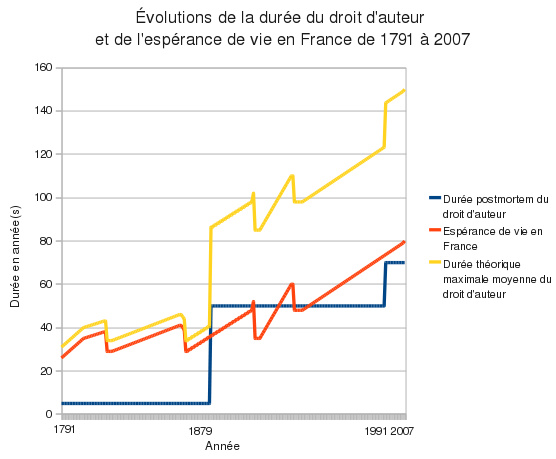
\includegraphics[scale=.85]{images/duree_du_droit_d'auteur_en_France_depuis_1791.png}
\caption{Évolution de la durée du droit d'auteur en France}
\end{figure}

Ces sociétés peut scrupuleuses font également appel à des méthodes d'intimidation pour faire toujours plus de profit.
L'astuce est de menacer d'attaquer en justice, pour violation du droit d'auteur/brevet détenu par la compagnie, des petites entreprises ou des particuliers.
Ceux-ci se voient alors offrir une porte de sortie, pour régler le différent <<~à l'amiable~>> : bien souvent le paiement d'une somme importante, mais moins importante et <<~risquée~>>\footnote{Risquée, car cette somme peut évoluer en fonction du verdict} que des frais de justice.
Il peut s'agir d'un coup de bluff, car le copyright/patent troll n'est pas obligé d'être sûr de gagner en justice : il lui suffit juste de le faire croire et d'intimider sa victime suffisamment pour que celle-ci choisisse d'elle même de régler ce différent fictif à l'amiable.

De telles entreprises sont un fléau pour la société, car elles cherchent à produire de la richesse en violant le système, mais surtout en obstruant la création !
C'est une des raisons pour lesquelles les systèmes du brevet et du droit d'auteur atteignent leurs limites : la société se retrouve à rémunérer la non-valeur ajoutée, ce qui est contraire à beaucoup de ses principes.

Dans le même ordre d'idées, certains n'hésitent pas à déposer des brevets tellement vagues ou évidents qu'ils peuvent alors potentiellement attaquer n'importe qui en justice pour violation de brevet.
Voici par exemple du smiley, issue du site \href{http://copyrightmadness.tumblr.com/}{CopyrightMadness} :

\begin{quotation}
\textit{<<~En Finlande, un troll de premier ordre a tenté d'enregistrer comme marque\dots{} le smiley.
Vous avez bien lu : la petite binette souriante de côté dont vous ponctuez vos tweets et vos emails ;-)
Fort heureusement, les juges qui avaient été saisis de cette demande ont estimé que les smileys ne pouvaient pas faire l'objet d'une telle protection et qu'ils devaient rester d'usage libre pour tous, y compris à des fins commerciales.
Un peu de Trademark Wisdom, ça fait du bien de temps en temps, mais sachez qu'en France, le smiley (la face jaune souriante, pas les signes typographiques) fait bien l'objet d'une protection, accordée à la famille Loufrani, qui en fait un usage particulièrement délirant :-(~>>}\footnote{Source : \url{http://storify.com/Copyrightmad/copyright-madness-du-1er-au-7-octobre}}
\end{quotation}

En parallèle de ces cas <<~extrêmes~>>, les entreprises qui, elles, produisent de la valeur n'hésitent pas non plus à utiliser le système à leur avantage, et, encore une fois, au désavantage du progrès et de la société.

On peut par exemple citer Apple, qui a décidé de breveter un concept, utilisé dans son iPhone, qu'on peut résumer par : <<~déverrouiller son téléphone en glissant son doigt sur une icône~>>.
Il parait complètement fou que ce brevet de 28 pages puisse exister et appartenir à quelqu'un.

Ce cas n'est pas isolé.
Un diagramme qui schématise les actions en justice pour violation de brevet dans le domaine des smartphones de 2008 à 2012 est disponible en annexe (page \pageref{annexe-smartphones}).

On peut voir que Apple est très impliqué dans ce genre d'affaires, que ce soit en tant que victime ou qu'agresseur.
Peu avant sa mort, Steve Jobs (co-fondateur et dirigeant de Apple pendant une longue période), a déclaré, à propos d'Android (système d'exploitation pour mobiles, principal concurrent du système pour iPhone, iOS) :

\begin{quote}
\textit{{\Large <<~I'm going to destroy Android, because it's a stolen product.
I'm willing to go thermonuclear war on this.~>>}}
\end{quote}

Ou, en français :

\begin{quote}
\textit{{\Large <<~Je vais détruire Android, car c'est un produit volé.
Je déclencherais une guerre thermonucléaire s'il le faut.~>>}}
\end{quote}

C'est à mettre en relation avec le fait que Apple ait copié les prototypes de Xerox, sans quoi nous ne connaitrions probablement même pas l'entreprise à la pomme.
En effet, la plupart des mécanismes que nous utilisons aujourd'hui sur n'importe quel ordinateur grand public ont été inventés par Xerox : souris, bureau, dossiers et fichiers, menus déroulants, \dots{}
En parlant de ça, Steve Jobs cite Picasso :

\begin{quote}
\textit{{\Large <<~Les bons artistes copient, les grands artistes volent.
~>>}
\begin{flushright}Pablo Picasso\end{flushright}}
\end{quote}

Si Xerox avait réagit comme Apple et ses concurrents réagissent de nos jours, nul doute que cette compagnie plus grande et plus mature n'aurait fait qu'une bouchée d'un Apple jeune et inexpérimenté\dots{}

%(copyright/patent troll, rémunération du non-ajout de valeur, appropriation d'idées communes, exemple Apple)
\section{Une histoire qui se répète ?}

Ces démonstrations d'agressivité et ces répressions à l'encontre des technologies de copie et de partage de l'information ne sont pas nouvelles.
Je vais survoler ici quelques exemples issus du passé, et nous verrons si l'Histoire peut nous enseigner une leçon.
Pour de plus amples détails, je recommande le 3\ieme{} chapitre (si ce n'est l'ensemble) du document <<~Sur la réforme du droit d'auteur~>>\footnote{\url{http://reformedroitauteur.sploing.fr/}}, sur lequel je me baserai pour écrire cette partie.

1450.
L'Europe se remet toujours de la Peste Noire, survenue à peu près un siècle plus tôt.
À cette époque, le moyen le plus simple pour obtenir une copie d'un livre est d'aller l'acheter à un moine.
Les moins-copistes présentent malheureusement beaucoup de désavantages :

\begin{itemize}
\item Ils ne publient que les livres acceptés par l'Église ;
\item ils ont besoin d'énormément de matières premières (environs 170 peaux de veau ou 300 de mouton) ;
\item même s'ils sont capables de corriger des fautes, ils en introduisent aussi de nouvelles ;
\item ils ne sont pas très nombreux (ils n'ont pas souffert directement de la peste, grâce à leur isolement, mais ne peuvent pas trop compter sur la population, qui elle en a souffert, pour renouveler leurs rangs).
\end{itemize}

1451.
Gutenberg améliore la presse à imprimer en la dotant de caractères mobiles.
Cette invention révolutionne la société.
Les moines-copistes sont rendus obsolètes.

L'Église catholique perd son monopole de l'information.
Elle tenta de faire pressions sur les rois pour bannir cette technologie.
Un des arguments qui fut avancé disait : <<~comment allons-nous payer les moines-copistes ?~>>
Elle réussit partiellement pendant un temps, lorsqu'en 1535 une loi fit fermer toutes les librairies et condamner \textbf{à mort} quiconque utilisait une imprimerie.
Finalement, l'Église catholique ne réussit pas à empêcher la propagation de l'imprimerie, laissant la voie libre à la Renaissance et au protestantisme, mais beaucoup de sang coulât pour empêcher la circulation rapide et efficace des idées, de la culture et de la connaissance.



%(exemples de "crises" similaires et résolues, exemple des bibliothèques)
\section{Interdire implique contrôler} % ou L'interdiction implique le contrôle
(DRM, HADOPI, DPI, cloud, vie privée, annexe vélo)
\section{Partager favorise le progrès}
% sanctionner copie = sanctionner inspiration (cf chap 1)
(les pirates achètent, exemple de Arduino, exemple de la mode)
